
\documentclass[12pt]{article}% Math and Physical Sciences 

\usepackage{graphicx}%
\usepackage{multirow}%
\usepackage{amsmath,amssymb,amsfonts}%
\usepackage{amsthm}%
\usepackage{mathrsfs}%
\usepackage[title]{appendix}%
\usepackage{xcolor}%
\usepackage{textcomp}%
\usepackage{manyfoot}%
\usepackage{booktabs}%
%\usepackage{algorithm}%
%\usepackage{algorithmicx}%
\usepackage{algpseudocode}%
\usepackage{listings}%
\usepackage{geometry}
\geometry{a4paper,left=2cm,right=2cm,top=1.7cm,bottom=1.7cm}
\usepackage{booktabs}
\usepackage{makecell}
\usepackage[ruled,longend,linesnumbered]{algorithm2e}
\usepackage{float}
\usepackage{natbib}


%% as per the requirement new theorem styles can be included as shown below
\theoremstyle{thmstyleone}%
\newtheorem{theorem}{Theorem}%  meant for continuous numbers
%%\newtheorem{theorem}{Theorem}[section]% meant for sectionwise numbers
%% optional argument [theorem] produces theorem numbering sequence instead of independent numbers for Proposition
\newtheorem{proposition}[theorem]{Proposition}% 
%%\newtheorem{proposition}{Proposition}% to get separate numbers for theorem and proposition etc.

\theoremstyle{thmstyletwo}%
\newtheorem{example}{Example}%
\newtheorem{remark}{Remark}%

\theoremstyle{thmstylethree}%
\newtheorem{definition}{Definition}%

\raggedbottom
%%\unnumbered% uncomment this for unnumbered level heads

\begin{document}

\title{Gaussian type observation error}

%%=============================================================%%
%% Prefix	-> \pfx{Dr}
%% GivenName	-> \fnm{Joergen W.}
%% Particle	-> \spfx{van der} -> surname prefix
%% FamilyName	-> \sur{Ploeg}
%% Suffix	-> \sfx{IV}
%% NatureName	-> \tanm{Poet Laureate} -> Title after name
%% Degrees	-> \dgr{MSc, PhD}
%% \author*[1,2]{\pfx{Dr} \fnm{Joergen W.} \spfx{van der} \sur{Ploeg} \sfx{IV} \tanm{Poet Laureate} 
%%                 \dgr{MSc, PhD}}\email{iauthor@gmail.com}
%%=============================================================%%


%%================================%%
%% Sample for structured abstract %%
%%================================%%

% \abstract{\textbf{Purpose:} The abstract serves both as a general introduction to the topic and as a brief, non-technical summary of the main results and their implications. The abstract must not include subheadings (unless expressly permitted in the journal's Instructions to Authors), equations or citations. As a guide the abstract should not exceed 200 words. Most journals do not set a hard limit however authors are advised to check the author instructions for the journal they are submitting to.
% 
% \textbf{Methods:} The abstract serves both as a general introduction to the topic and as a brief, non-technical summary of the main results and their implications. The abstract must not include subheadings (unless expressly permitted in the journal's Instructions to Authors), equations or citations. As a guide the abstract should not exceed 200 words. Most journals do not set a hard limit however authors are advised to check the author instructions for the journal they are submitting to.
% 
% \textbf{Results:} The abstract serves both as a general introduction to the topic and as a brief, non-technical summary of the main results and their implications. The abstract must not include subheadings (unless expressly permitted in the journal's Instructions to Authors), equations or citations. As a guide the abstract should not exceed 200 words. Most journals do not set a hard limit however authors are advised to check the author instructions for the journal they are submitting to.
% 
% \textbf{Conclusion:} The abstract serves both as a general introduction to the topic and as a brief, non-technical summary of the main results and their implications. The abstract must not include subheadings (unless expressly permitted in the journal's Instructions to Authors), equations or citations. As a guide the abstract should not exceed 200 words. Most journals do not set a hard limit however authors are advised to check the author instructions for the journal they are submitting to.}



%%\pacs[JEL Classification]{D8, H51}

%%\pacs[MSC Classification]{35A01, 65L10, 65L12, 65L20, 65L70}

\maketitle

\section{Recap how likelihood works in UQlab}\label{sec1}

We assume the discrepancy model follow Gaussian distribution with unknown residuals $\boldsymbol{\epsilon}$. Likelihood function can be expressed as:

\begin{equation}        
        \label{eq: Likelihood function}
        \begin{aligned}
         \mathcal{L}(\boldsymbol{\theta}|\mathcal{Y}) =& \prod_{i=1}^{N} N(\boldsymbol{y_{i}}|\mathcal{M}(\boldsymbol{\theta}),\boldsymbol{\Sigma}) \\
         =& \prod_{i=1}^{N}\frac{1}{\sqrt{(2 \pi)^{N_{\rm{out}}}{\rm{det}} 
         (\boldsymbol{\Sigma})}}\exp\left(-\frac{1}{2}\left(\boldsymbol{y_i} - \mathcal{M}(\boldsymbol{\theta})\right)^{\mathsf{T}} \boldsymbol{\Sigma}^{-1}\left(\boldsymbol{y_i} - \mathcal{M}(\boldsymbol{\theta})\right)\right) 
        \end{aligned}
        \end{equation}


Because $\boldsymbol{\epsilon}$ is unknown, it is considered in the prior $\vec\theta$ with predefined distribution $\boldsymbol{\epsilon} \sim \mathcal{N}(0,\sigma^2)$. $\vec\theta$ is a vector of parameters of interests (soil parameters and $\boldsymbol{\epsilon}$).\\


\textbf{Note:} All measurement data points or covariance matrix $\boldsymbol{\Sigma}^{-1}$ default in UQLAB share i.i.d. assumption, i.e., all discrepancy models of the multiple points hold the same prior and $\sigma^2$. 


$\boldsymbol{\epsilon}$ is non-informative, thus, its prior for the variance follows uniform distribution $\sigma\sim \mathcal{U}$(0,$\sigma_{0}^2$), in which $\sigma_{0}^2$ should be related to the observation values. 

UQLAB suggests (as I see) adopting its mean value of the monitored data points along the simple beam problem. Also UQLAB assume the  the covariance matrix at different locations has no influence on the monitored data error (i.e., iid assumption mentioned above).


Tricky part is how to relax the iid assumption in UQLAB's custom likelihood. Wagner(2020) recommands hyperparameters $\boldsymbol{w}$.

\section{How Wagner handle non-diagonal covariance matrix}

Relax iid:

\begin{equation}
        \Sigma_{ij} = \sigma_{i}\sigma_{j}R \\
        \end{equation}
        \begin{equation}
           \boldsymbol{\sigma} = (\sigma_1,...,\sigma_N) \\ 
        \end{equation}
        \begin{equation}
\sigma_{i} = \sum_{k=0}^{6} \omega_{k} \times \psi_{k} 
        \end{equation}

In this way, $\boldsymbol{w}_{k}$ should be related with obeservation. Therefore, Wagner adopts prior as Figure \ref{fig:w}:
\begin{figure}[H]
    \centering
    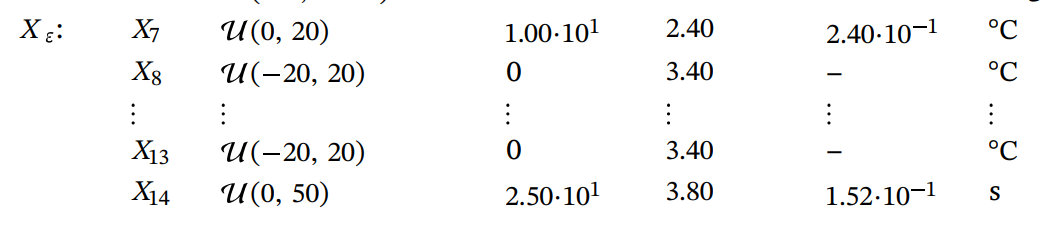
\includegraphics[width = 10cm]{w_prior.png}
    \caption{Priors for $\boldsymbol{w}_{k}$}
    \label{fig:w}
\end{figure}

The prior's in Figure $\ref{fig:w}$ values is related with observation and it is set as 20. It is reasonable and easy to implement becasue Wagner is not doing sequential updating and need the prior only once. But when it comes to multiple stages, manually selecting the priors related with observations is troublesome. In another word, hyperparameters in Wagner's paper have units.






\section{How we handle this}

Based on Wagner's paper, we make the hyper parameters $\boldsymbol{w}_{k}$ as a normalized value to get rid of the units.

\begin{equation}
        \Sigma_{ij} = \sigma_{i}\sigma_{j}R \\
        \end{equation}
        \begin{equation}
           \boldsymbol{\sigma} = (\sigma_1,...,\sigma_{101}) \\ 
        \end{equation}
\begin{equation}
    y_{j} = max(\mathcal{Y}_{obs\_j})
\end{equation}
        \begin{equation}
\sigma_{i} = \sum_{k=0}^{6} \omega_{k} \times \psi_{k} \times y_{j}; i = \{1,\cdots,101\}
        \end{equation}

in which, $\mathcal{Y}_{obs\_j}$ is observation for  loading stage  $j$; $\mathcal{Y}_{obs\_j} = \{ y_1,y_2,...,y_{101}\}$; for example, $\mathcal{Y}_{obs} = \{\mathcal{Y}_{obs\_1},...,\mathcal{Y}_{obs\_9}  \}$ for 9 loading stages, $R$ is constant as 1 not considering non-diagonal effect.

In this way, the only prior we need to control is now only normalized $\boldsymbol{w}_{k}$ without units.


\begin{algorithm}
    \caption{Gaussian type observation error} \label{alg:loglikelihood}

\KwData{hyperparams prior $\boldsymbol{w}$; observations $\mathcal{Y}_{obs}$}
\KwResult{Observation erro covariance $\boldsymbol{\Sigma}$}

Initialization\; 

$E \gets params(:,1); \delta \gets params(:,2); \epsilon \gets params(:,3)$; \# Array of variables from $params$ \; 

$Nchain \gets$ Number of rows from $params$, i.e., MCMC chains \; 

$Nexp \gets$  Number of rows from $Y$, i.e., number of experiments \; 

\For{$i \gets 1 \ to  \ Nchain$}{

    \For{$ j \gets 1 \ to \ Nexp$}{
    $\Delta \ell{\mathcal{L}}(i,j)$ = $-\frac{1}{2}\left(\boldsymbol{Y(i,j)} - \mathcal{M}(\vec\theta)\right)^{\mathsf{T}} \boldsymbol{\Sigma}^{-1}(\epsilon)\left(\boldsymbol{Y(i,j)} - \mathcal{M}(\vec\theta)\right) 
    - \frac{1}   {2}\ell\det((\boldsymbol{\Sigma}(\epsilon))$\;

 $\ell{\mathcal{L}}(i)$ $\gets$  $\ell{\mathcal{L}}(i)$+ $\Delta \ell{\mathcal{L}}(i,j)$ \;
    $j = j +1$;\
}
    $i = i +1$
}

\end{algorithm}

\end{document}
